\documentclass[a4paper,12pt]{ctexbeamer}
\usetheme{CambridgeUS}
\usepackage{amsmath}
\usepackage{amsfonts}
\usepackage{float}
\usepackage{enumerate}
\usepackage{svg}
\usepackage{graphicx}
\usepackage{booktabs}
\usepackage{hyperref}
\usepackage[style = gb7714-2015ay, url=false,gbtitlelink=true]{biblatex}
\addbibresource{thesis.bib}
\title[开题报告]{极端天气冲击对风险偏好的影响——以家财险需求为例}
\author{董晨阳}
\date{\today}
\renewcommand{\bibfont}{\normalfont\small}
\begin{document}
\AtBeginSection[]
{
    \small
    \begin{frame}
        \frametitle{目录}
        \tableofcontents[
            sectionstyle=show/shaded,
            subsectionstyle=show/show/hide,
            subsubsectionstyle=show/show/show/hide
        ]
    \end{frame}
}
\maketitle
% 2、内容:包括选题来源、研究意义、国内外研究状况、主要研究内容、拟采取的研究方法、预期研究结果和论文写作计划等。
\section{研究背景与意义}
\begin{frame}
    \frametitle{研究背景:极端天气频发}

    在现代社会,气候变化已经成为一个备受瞩目的全球性问题。在灾害面前,家庭往往是首当其冲的受害者。但与企业相比,个人家庭对这些潜在风险的反应可能更为复杂。家庭是否会通过购买家财险来缓解财产损失,以及他们在灾害发生后是否更加倾向于购买保险,这些问题有许多影响因素,具有较强的实证研究价值。
    \begin{table}[H]
        \centering
        \caption{今年来全球极端天气}
        \tiny
        \begin{tabular}{lll}
            \toprule
            事件       & 时间                    & 死亡人数                            \\
            \midrule
            丹尼尔风暴    & 9月4日–12日              & \textgreater{}4,034+(10,100+失踪) \\
            弗雷迪飓风    & 2月5日–3月14日            & 1,434                           \\
            摩卡飓风     & 5月9日–15日              & 438(+101失踪)                     \\
            阿富汗寒潮    & 1月10日–17日             & 166                             \\
            西北美洲热浪   & 5月–至今                 & \textgreater{}112               \\
            北印度洪水    & 7月10日–至今              & \textgreater{}100               \\
            菲律宾洪水    & 2022年12月18日–2023年2月5日 & 97(+25失踪)                       \\
            圣保罗洪水和滑坡 & 2月18日–23日             & 65(+58失踪)                       \\
            巴基斯坦洪水   & 6月22日–7月6日            & 54                              \\
            奥蒂斯飓风    & 10月22日–25日            & 50–350                          \\
            \bottomrule
        \end{tabular}
    \end{table}
\end{frame}

\begin{frame}
    \frametitle{研究背景:巨灾可能对风险偏好有所影响}
    巨灾频繁发生给人们造成物质上的创伤同时,也对人们的风险偏好有着潜移默化的影响,例如位于台风路径上的企业更偏好持有现金\citep{杨娜娜2019自然灾害与企业现金持有}。\textbf{极端天气冲击对人们风险偏好是否会产生影响以及产生何种影响是一个值得研究的课题,能帮助我们提前做好风险管理措施,而不是总是亡羊补牢}。

    2023年10月24日,我国政府宣布增发2023年国债1万亿元,集中用于灾后恢复重建和提升国家防灾减灾能力。这一决策表明政府对气候变化带来的灾害风险的高度关注,也突显了防灾减灾工作的紧迫性。
\end{frame}

\begin{frame}
    \frametitle{研究主题:极端天气冲击对家财险需求的影响}
    我国的家财险始于1980年,我国财产保险的早期发展同时也是家庭财产保险演进的历史\citep{黄英君2008论我国产险公司分散性业务营销模式的创新},塑造了国人对财产险最早的认知。

    然而,极端天气下人们对自身及财产安全的关切是否能够转化为保险需求是一个相对较少被深入研究的领域。本研究的选题来源于对这一领域的关注,力图了解极端天气极端冲击对风险偏好的影响,填补现有研究的空白。
    \begin{figure}[H]
        \centering
        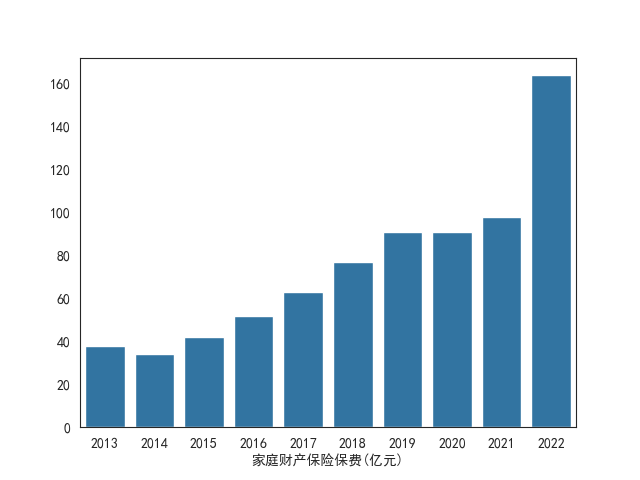
\includegraphics[width=0.6\linewidth,trim=0 0 0 40]{img/家庭财产保险保费.png}
    \end{figure}
\end{frame}

\begin{frame}{研究意义}
    \begin{enumerate}
        \item 通过深入研究极端天气对家财险需求的影响,我们能够为保险公司提供更为精准的市场预测
        \item 研究结果还可以为政府和监管机构提供政策制定的依据,为
        \item 研究家财险需求的变化还能够提供社会科学领域对于人类行为和决策的深刻洞察
        \item 可持续发展的角度来看,本研究有助于引导人们更加理性和科学地对待气候变化风险
    \end{enumerate}
\end{frame}


\section{文献综述}

\subsection{极端天气冲击对不同种类保险需求的影响}
\begin{frame}
    \frametitle{极端天气冲击对健康险需求的影响}
    \begin{itemize}
        \item 空气污染水平对健康险的购买或退保的决策产生的显著影响\citep{2018Something},每日空气污染水平每增加一个标准差,当天销售的保险合同数量增加了7.2\%。而在考虑购买后的条件下,即在冷静期内,相对于订单日期水平,每日空气污染水平每减少一个标准差,退保概率增加了4.0\%,研究还探讨了多种可能的机制,发现了对投射偏差和显著性的最有力支持。
        \item 空气污染对中国居民商业健康保险需求的影响大小\citep{赵强2021空气污染对商业健康保险需求的影响},利用2011年至2016年秦岭淮河地区84个地级市的宏观数据,采用模糊断点回归设计和中国北方集中供暖政策的准自然实验方法,发现空气污染对商业健康险需求存在显著的正向影响,特别是PM2.5污染物的排放浓度每提升1\%,商业健康保险密度提高1.098\%。
    \end{itemize}
\end{frame}
\begin{frame}
    \frametitle{极端天气冲击对健康险需求的影响机制}
    \begin{itemize}
        \item 空气污染提升了个人的风险感知,进而引起健康保险需求增加\citep{宋平凡2022空气污染}。基于2006—2016年中国283个地级以上城市的数据,系统考察了空气污染对健康保险需求的实证影响,采用百度指数作为风险感知的代理变量,并运用中介效应模型验证了空气污染对健康保险需求的影响机制。结果显示,通过百度指数体现的风险感知效应是空气污染引起健康保险需求增加的重要途径,并且工具变量中介效应模型的实证结果进一步支持了这一结论。
        \item 气候变化增加了居民对气候风险和健康的关注\cite{zhong2022exposure}。增加了居民对气候风险的关注,使其更倾向于购买健康保险以规避潜在的健康风险;异常高温对健康的实质性影响也使居民更加关注自身的医疗保障需求。
    \end{itemize}
\end{frame}

\begin{frame}
    \frametitle{极端天气对寿险需求影响}
    \begin{itemize}
        \item 欧盟成员国研究保费金额和温室气体排放的关系\citep{melnychenko2021influence},结果表明每千吨温室气体排放的增加导致寿险保费金额增加17万欧元,具有显著性。
        \item 影响机制方面,有观点研究2013年德国洪水对个人的冲击\citep{avdeenko2021impact},认为这种变化是风险厌恶选择导致高风险地区人寿保险需求的增加,通过幸福感的变化来介导,从而解释了风险偏好的改变。
    \end{itemize}
\end{frame}

\begin{frame}
    \frametitle{极端天气对财产险需求影响}
    近年来天气灾害致汽车出险的数量明显增加\citep{张翠华2020天气灾害致车险理赔的风险分析},其研究数据集为河北省2004-2018年天气灾害致车险理赔事故,研究发现主导汽车出险的天气灾害主要包括暴雨、涉水、冰雹和暴风,在不同地区出险数量存在明显的差异。
\end{frame}

\begin{frame}
    \frametitle{极端天气对农险需求影响}
    \citet{胡新艳2021气候变化}通过地级市气候数据和农户微观数据进行匹配,进行了实证分析。研究发现,气候变化在显著促进农户农业保险购买行为方面发挥了关键作用,但在不同生产目的的农户中存在异质性影响。

    具体而言,当农户的经营目标从满足自家消费转向为追求市场利润时,其购买农业保险的需求更为强烈。进一步分析表明,气候变化导致的两类农业风险对农户购买农业保险的中介作用存在差异。土壤退化风险由于具有渐进性,农户能够在农业生产之前通过调整生产要素供给来降低风险损失,因此对农业保险的需求较为低迷。相反,病虫害风险属于突发性风险,农户难以通过事前风险防控来分散风险,从而强化了其对农业保险的需求。
\end{frame}


\subsection{风险偏好的影响因素}
\begin{frame}
    \frametitle{风险偏好与商业保险购买之间存在正向关系}
    \begin{itemize}
        \item \citet{宋章良2021我国中老年家庭风险偏好对商业保险购买行为的影响研究}认为正向关系的主要原因在于,即高风险偏好的家庭更倾向于购买投资型保险而非保障型保险,与此同时该群体的人均收入较高。
        \item \citet{孙武军2023商业健康保险的配置能够改变家庭的风险偏好吗}认为购买商业保险也会改变家庭风险偏好,家庭配置商业健康保险能够显著提高家庭的主客观风险偏好。此外,通过对异质性分析的深入研究,发现这种正面影响在低收入家庭中尤为显著,而在高收入家庭中则作用较为微弱。
    \end{itemize}
\end{frame}

\begin{frame}
    \frametitle{自然灾害会对风险偏好产生影响}
    有研究以中国2003-2005年发生的4次地震为案例,利用国家统计局城镇住户调查数据,通过双重差分法的研究方法,探讨地震对城镇家庭风险偏好的影响及其背后的机制\citep{章元0地震冲击对风险偏好的影响}。地震显著提高了城镇家庭的风险厌恶程度。尤其是距离震中越近的家庭,在地震发生后,购买彩票的概率和支出下降越为显著。这一结果揭示了地震引起的风险预期上升和负向情绪冲击是重要的机制。进一步分析显示,距离震中越近的家庭,其震后非储蓄性保险支出以及用于缓解负向情绪的消费支出上升越多。这意味着地震对家庭风险偏好的影响,不仅体现在经济决策上,还体现在对非储蓄性保险和消费行为的调整上。
\end{frame}
\begin{frame}
    \frametitle{其他风险偏好影响因素方面}
    \begin{enumerate}
        \item 收入\citep{石双2018收入与风险偏好}
        \item 资产总额\citep{卢亚娟殷君瑶2021户主风险态度对家庭金融资产配置的影响研究}
        \item 年龄\citep{王晶2021年龄结构}
        \item 健康状况\citep{雷晓燕2010中国家庭的资产组合选择}
        \item 教育程度\citep{梁立俊2018受教育程度与主客观风险偏好}
        \item 职业\citep{赵颖2017中国劳动者的风险偏好与职业选择}、性别\citep{徐小华2019女性劳动参与会影响家庭资产配置风险偏好吗}
    \end{enumerate}
\end{frame}

\section{未来研究计划}


\begin{frame}{主要研究内容与拟采取的研究方法}
    本文计划研究气候变化对家庭财产保险需求的影响机制,主要研究内容包括:

    \begin{enumerate}
        \item 气候变化是否影响家庭财产保险需求,如果影响,影响程度如何
        \item 气候变化对家庭财产保险需求的影响机制,可能的影响因素包括:气候变化通过影响家庭风险偏好影响保险需求、气候变化对家庭财产损失频率的影响、气候变化对家庭财产损失程度的影响等
        \item 家庭风险偏好对气候变化影响下家庭财产保险需求的调节作用,例如风险偏好越高,家庭财产保险需求的增加是否越显著
    \end{enumerate}
\end{frame}


\begin{frame}{预期研究结果}
    本文预期研究结果包括:

    \begin{enumerate}
        \item 气候变化对家财险需求具有显著性影响,可以看到地震、洪水、火灾等气候异常现象发生后,家庭财产保险需求会显著增加
        \item 气候变化对家庭财产保险需求的影响机制是否成立,异质性检验结果显示,气候变化通过影响家庭风险偏好影响保险需求、气候变化对家庭财产损失频率的影响、气候变化对家庭财产损失程度的影响等都是影响机制
        \item 家庭风险偏好对气候变化影响下家庭财产保险需求具有一定的的调节作用
    \end{enumerate}
\end{frame}
\begin{frame}{论文写作计划}
    \begin{enumerate}
        \item 一月前完成数据的清洗和描述性统计分析
        \item 二月前完成模型的建立和实证分析
        \item 三月前完成论文的初稿
        \item 四月前完成论文的修改和定稿,同时不断阅读文献寻找新思路
    \end{enumerate}
\end{frame}



\appendix
\nocite{*}
\begin{frame}[allowframebreaks]
    \frametitle{参考文献}
    \tiny{\printbibliography}
\end{frame}
\end{document}
